\documentclass[11pt,letterpaper]{article}
\usepackage[margin=0.77in,headheight=15pt]{geometry}
\usepackage{amsmath,booktabs,graphicx,array,tabularx,xcolor,fancyhdr,caption,float}
\usepackage[hidelinks]{hyperref}
\definecolor{navy}{HTML}{17384D}
\definecolor{muted}{HTML}{52616B}
\newcolumntype{Y}{>{\raggedright\arraybackslash}X}
\newcolumntype{P}[1]{>{\raggedright\arraybackslash}p{#1}}
\setlength{\parindent}{0pt}
\setlength{\parskip}{5pt}
\setlength{\tabcolsep}{5pt}
\setlength{\emergencystretch}{2em}
\renewcommand{\arraystretch}{1.13}
\captionsetup{font=small,labelfont=bf}
\graphicspath{{images/}}
\pagestyle{fancy}
\fancyhf{}
\fancyhead[L]{\small\color{muted}SONIC sound-delivery bench}
\fancyhead[R]{\small\color{muted}23 October 2026}
\fancyfoot[L]{\small\color{muted}Saved-data analysis | Revision 1}
\fancyfoot[R]{\small\thepage}
\renewcommand{\headrulewidth}{0.3pt}
% Generated from measured verification records.
\newcommand{\DelayMedian}{38.307}
\newcommand{\DelayMinimum}{38.240}
\newcommand{\DelayMaximum}{38.375}
\newcommand{\DelaySpan}{0.135}
\newcommand{\RunMedianShift}{0.125}
\newcommand{\AcceptedSweepBands}{84}
\newcommand{\TotalSweepBands}{101}
\newcommand{\SupportedLowHz}{158.74}
\newcommand{\SupportedHighHz}{13561.13}

\begin{document}

{\LARGE\bfseries\color{navy} Full bench analysis report}\par\vspace{5pt}
{\large Speaker playback, microphone recording, timing and frequency response}\par\vspace{3pt}
{\small SONIC Auditory Benchmarking \hfill Data acquired 23 October 2026}

\section{Findings and decision summary}
The wired playback and microphone-recording path is operational. Analysis of four
saved native captures establishes a repeatable \emph{application sample-grid waveform
roundtrip} of approximately \textbf{38.3 ms} with nonperiodic timing probes.
Both SONIC recordings contain components at every requested Sheep E frequency,
but their recorded levels are substantially unequal. These findings support a
working bench demonstration; they do not yet qualify calibrated delivery across
the full SONIC alphabet.

\begin{table}[H]
\small
\begin{tabularx}{\linewidth}{@{}P{0.28\linewidth}Y@{}}
\toprule
Question & Finding from the saved data\\
\midrule
Playback and recording together? & Verified by the known-melody check and the two recorded SONIC blocks.\\
Measured roundtrip? & Forty of forty sweeps accepted. Pooled median \DelayMedian\,ms; observed range \DelayMinimum--\DelayMaximum\,ms.\\
Repeatability? & Two stream-start medians: 38.250 and 38.375\,ms. Their difference is \RunMedianShift\,ms.\\
All 14 SONIC components? & Observed in both microphone recordings, with control and neighboring-tone checks. This is recorded pickup, not isolated acoustic qualification.\\
Uniform frequency level? & Not established. Relative to 2\,kHz, 17--19.5\,kHz was about 15--22\,dB lower; 20.9--25.8\,kHz about 30--40\,dB lower.\\
SPL, distortion, acoustic onset? & Unqualified: microphone correction, absolute level calibration, acoustic-isolation controls and independent physical timing were not available.\\
\bottomrule
\end{tabularx}
\caption{Main conclusions. Numeric delays refer to the sweep-based application roundtrip, not a delay measured directly from SONIC tones.}
\end{table}

\textbf{Physical chain.} Computer/Core Audio $\to$ Audient iD14 $\to$ wired Edifier
speaker path $\to$ air $\to$ Earthworks M50 $\to$ Audient microphone input 1 $\to$
the recording program. The operator reported approximately 10\,cm separation.
The exact acoustic reference plane, orientation and active cabinet assignment were
not independently measured. Host outputs 1 and 2 received the same mono array;
which physical speaker or speakers reproduced it was not fully logged.

\textbf{Report scope.} This is an offline review of existing recordings. No new
playback, acquisition or hardware change was performed for this report. No neural
or animal data were collected. Derived figures and records are publishable project
artifacts; raw room audio remains local. The measured records are the evidence
base, rather than the browser demonstration or manufacturer bandwidth claims
\cite{delay,pip,sweep,basic}.

\newpage
\section{Dataset, acquisition and stimulus provenance}
The principal dataset comprises two timing-probe captures and two SONIC E14
captures: \textbf{195.2 seconds} of native recording in four separately opened
full-duplex streams. All four passed the saved transport checks; all recorded
callback status flags were zero and no microphone sample reached the analysis
clipping threshold of $|x|\geq0.999$ full scale.

\begin{table}[H]
\centering\small
\begin{tabular}{@{}llrrrr@{}}
\toprule
ID & Stimulus & Events & Time (s) & Frames & Mic peak (dBFS) \\
\midrule
D1 & Timing sweeps & 20 & 11.6 & 1,113,600 & -25.50 \\
D2 & Timing sweeps & 20 & 11.6 & 1,113,600 & -25.46 \\
S1 & E14 block & 8,400 & 86.0 & 8,256,000 & -27.65 \\
S2 & E14 block & 8,400 & 86.0 & 8,256,000 & -30.41 \\
\bottomrule
\end{tabular}

\caption{Main captures at 96,000 samples/s. SONIC capture duration includes one second of silence before and after each 84-second stimulus block. Captured peak levels are digital dBFS, not dB SPL.}
\end{table}

\begin{tabularx}{\linewidth}{@{}lY@{}}
D1 & \path{20261023-155401}\\
D2 & \path{20261023-155500-roundtrip-repeat}\\
S1 & \path{20261023-155615-sonic-e14-full}\\
S2 & \path{20261023-160447-sonic-e14-full}\\
\end{tabularx}

\subsection{Acquisition configuration}
The program used a named Audient iD14 device through Core Audio and
\texttt{sounddevice} 0.5.6, with NumPy 2.3.5. Input channels 1/2 and output
channels 1/2 were opened together at 96\,kHz with float32 buffers, requested low
latency and automatic block size. Timing runs used 908-frame callbacks. The exact
source array, two-channel input array and per-buffer ADC/DAC timestamps were saved.
The primary response is microphone input 1. Input 2 was \emph{not} a validated
electrical timing reference in these successful captures.

Input monitoring was kept attenuated in the working mixer setup. The microphone
worked with the photographed switch configuration; phantom voltage, microphone
gain, monitor attenuation, cabinet EQ and complete hardware routing were not
numerically verified. No interface firmware update was performed, and its installed
version was not recorded. These omissions limit exact physical reproduction.

\subsection{Two distinct stimulus families}
\textbf{Timing probes (D1/D2):} twenty 100\,ms logarithmic sweeps from 100\,Hz
toward 20\,kHz, with 20\,ms raised-cosine end ramps, 500\,ms onset spacing, and
one-second padding. These locally specified probes are not SONIC stimuli.

\textbf{SONIC reconstruction (S1/S2):} 14 frequencies, in kHz,
\[
\{2,4,6,8,9,10.5,17,18.2,19.5,20.9,22.4,24,25.8,27\}.
\]
Each 10\,ms sine pip starts at zero phase and includes 2\,ms ramps at both ends,
with no silence between pips. Each block has 600 of every frequency: 8,400 pips
and 84 seconds. A PCG64 shuffle with seed 20261023 generated the order; the same
sequence was replayed in S2. Sources used $-24$\,dBFS nominal digital peak.
The frequency alphabet, pip duration, ramp duration and zero-phase convention
follow the paper's Sheep E specification. The ramp shape, seed/order, exact counts,
digital level and 96\,kHz rate are declared local reconstruction choices, not
original supplied SONIC audio \cite{sonic,pip}.

\newpage
\section{Timing analysis and results}
\subsection{The measured quantity}
Let $o$ be a source-array sample position and $i$ the matching microphone-array
position. The input/output array counters advance together in the native callback,
but equal indices do not represent simultaneous ADC and DAC events. The estimated
roundtrip is
\[
\widehat{D}_{\mathrm{app}}=\frac{i-o}{96{,}000}\,1000\ \mathrm{ms}.
\]
This sample-grid metric includes playback and recording buffering, interface
conversion, speaker response, propagation and the microphone path. It is not a
timed UI click, isolated speaker delay, first acoustic arrival or physical-only
DAC-to-ADC latency. Reported driver latency and host timestamps were not added
to or subtracted from it. PortAudio distinguishes requested/reported latency and
backend-dependent timing behavior; metadata alone does not independently calibrate
the physical chain \cite{portaudio,delay}.

Each exact 100\,ms probe was matched to the microphone with normalized waveform
cross-correlation over a causal 0--100\,ms lag search. Absolute correlation permits
polarity inversion. The existing screen rejected weak, clipped, ambiguous or
search-boundary matches and invalid transport. Local thresholds were $|r|\geq0.35$,
RMS above $10^{-6}$ full scale, and secondary-to-primary peak ratio below 0.95 after
excluding the primary correlation lobe. These are analysis screens, not approved
experimental acceptance limits.

\begin{table}[H]
\centering\small
\begin{tabular}{@{}lrrrr@{}}
\toprule
Run & Accepted & Median (ms) & Range (ms) & $|r|$ range \\
\midrule
D1 & 20/20 & 38.250 & 38.240--38.250 & 0.431--0.438 \\
D2 & 20/20 & 38.375 & 38.365--38.375 & 0.433--0.438 \\
\bottomrule
\end{tabular}

\caption{Sweep-based waveform roundtrip. The pooled median is \DelayMedian\,ms, with \DelaySpan\,ms total observed span. The two clusters correspond to separate stream starts.}
\end{table}

\begin{figure}[H]
\centering
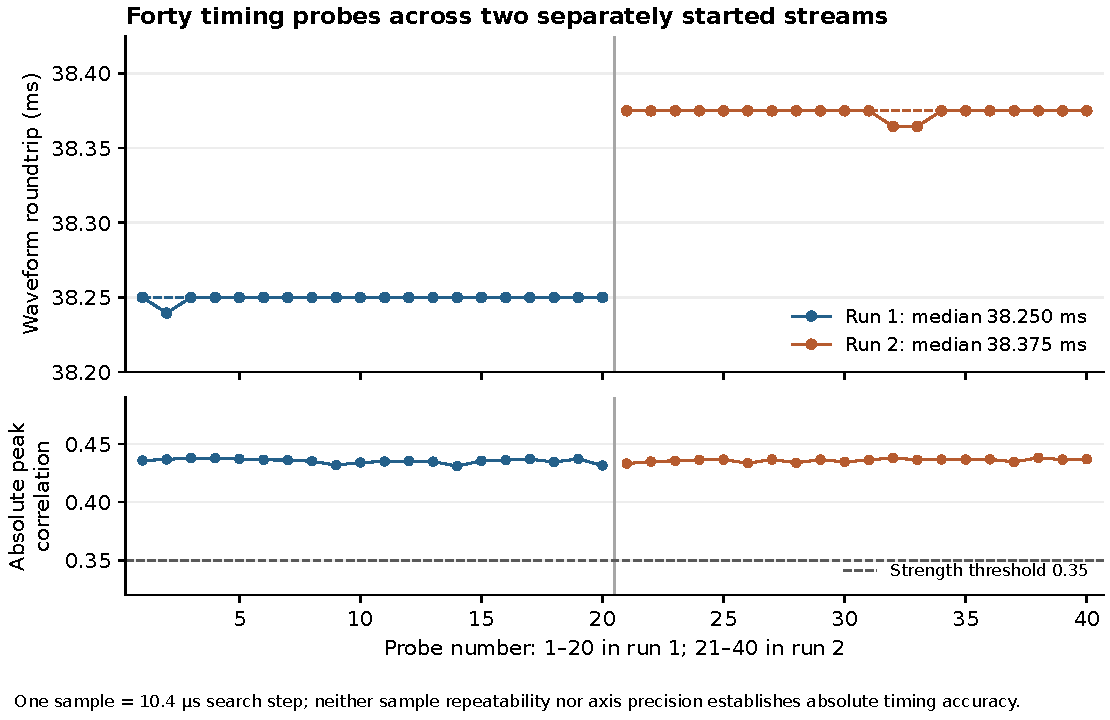
\includegraphics[width=.89\linewidth,height=.31\textheight,keepaspectratio]{TimingSummary.pdf}
\caption{All 40 accepted integer-sample delay estimates and their correlation strength. Points are measured values; no confidence interval or calibrated accuracy bound is implied. Each run spans one sample in detected peak position.}
\end{figure}

\newpage
\subsection{Waveform evidence and timing interpretation}
\begin{figure}[H]
\centering
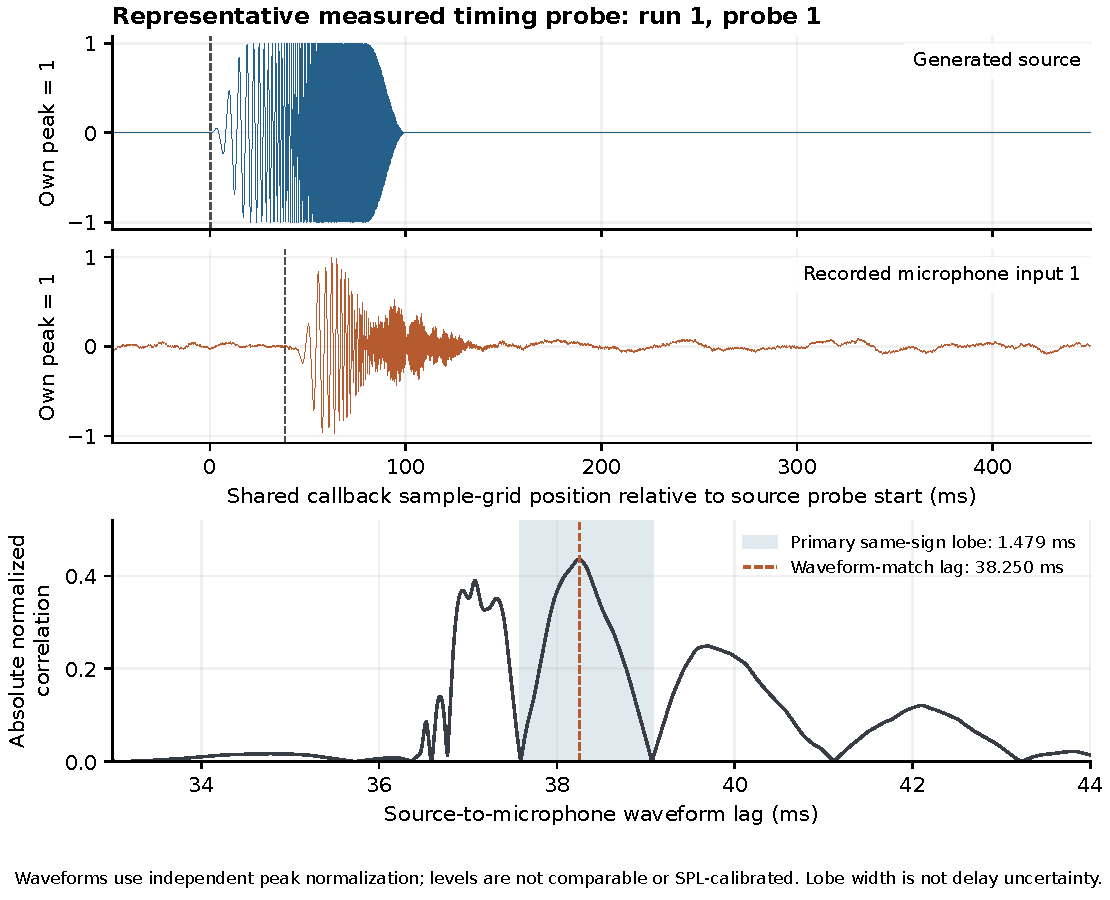
\includegraphics[width=.94\linewidth,height=.44\textheight,keepaspectratio]{ProbeWaveformCorrelation.pdf}
\caption{D1, first probe: actual source and microphone waveform in the application sample grid, followed by a zoom of the absolute normalized correlation. Trace amplitudes are normalized independently for display. The indicated correlation-lobe width is a shape diagnostic, not an uncertainty interval or first-arrival estimate.}
\end{figure}

Primary lobes spanned 141--142 samples (1.469--1.479\,ms). Within-run peak
positions varied by one sample (10.417\,$\mu$s), whereas run medians shifted
by 0.125\,ms. Small sample-grid variation demonstrates repeatability of the
estimator under this short test. It does not establish matching absolute accuracy:
filtering, multipath, frequency-dependent phase and waveform choice can move the
correlation maximum. Interpolated percentiles below one sample must not be reported
as sub-sample timing accuracy.

\textbf{Direct SONIC timing was not qualified.} Five four-second windows from the
recorded randomized tone sequence were tested separately. Four retained competing
carrier peaks above the 0.95 ambiguity ratio; only one passed. The minimum accepted
window screen was not met, so no SONIC-specific delay is reported. The
38.3\,ms result is the separate nonperiodic-sweep estimate \cite{playback}.

\textbf{Cadence and latency are different.} At 96\,kHz, a 10\,ms pip is 960 samples.
A precomputed sequence can stream at that cadence while a pipeline has an
approximately 38\,ms roundtrip. Neither fact demonstrates accurate sub-millisecond
acoustic pulses or synchronization to a neural recorder. Subtracting a fixed
offset in software also does not remove physical latency.

\newpage
\section{SONIC tone pickup and frequency-dependent level}
\subsection{Analysis of the actual short-pip recordings}
For every frequency in each block, a Hann-weighted complex projection measured
the component at the commanded frequency in a 576-sample (6\,ms) window. The
window covers source-relative 2--8\,ms after an approximate 38\,ms content shift:
\[
a_f=\frac{2\sum_n x[n]w[n]e^{-j2\pi fn/F_s}}{\sum_n w[n]},
\qquad A_{f,\mathrm{RMS}}=\frac{|a_f|}{\sqrt{2}}.
\]
The projection is a descriptive component estimate, rather than an isolated
steady-tone measurement. The 38\,ms shift locates content; it is not a
per-frequency delay result. Repeating extraction at 37 and 39\,ms measures
sensitivity to this local choice. Windowing reduces spectral leakage at the cost
of finite resolution; it does not remove neighboring-tone or ringing effects
\cite{ni,pip}.

\begin{table}[H]
\centering\small
\begin{tabular}{@{}rrrrrr@{}}
\toprule
\shortstack{Tone\\(kHz)} & \shortstack{S1 relative\\(dB)} & \shortstack{S2 relative\\(dB)} & \shortstack{S2--S1\\(dB)} & \shortstack{Min. contrast\\(dB)} & \shortstack{Alignment span\\(dB)} \\
\midrule
2 & 0.00 & 0.00 & +0.00 & 49.4 & 0.46 \\
4 & -2.70 & -2.68 & +0.01 & 52.1 & 0.56 \\
6 & -8.50 & -8.52 & -0.02 & 52.8 & 0.78 \\
8 & -7.36 & -7.24 & +0.12 & 55.9 & 0.61 \\
9 & -11.36 & -11.79 & -0.43 & 52.7 & 0.89 \\
10.5 & -8.66 & -8.59 & +0.07 & 58.1 & 0.85 \\
17 & -14.87 & -14.75 & +0.12 & 55.4 & 0.76 \\
18.2 & -18.62 & -18.73 & -0.12 & 52.2 & 0.82 \\
19.5 & -21.83 & -22.14 & -0.31 & 48.3 & 0.63 \\
20.9 & -40.36 & -37.70 & +2.66 & 31.9 & 5.90 \\
22.4 & -29.74 & -30.22 & -0.47 & 41.0 & 0.43 \\
24 & -36.80 & -38.34 & -1.54 & 10.5 & 0.62 \\
25.8 & -37.13 & -35.44 & +1.69 & 32.9 & 1.46 \\
27 & -28.59 & -28.69 & -0.09 & 39.1 & 0.54 \\
\bottomrule
\end{tabular}

\caption{All-target medians, 600 pips/frequency/capture. Levels are relative to the same capture's 2-kHz median. Minimum contrast is the lowest pre-block or other-tone contrast across S1/S2, in amplitude-ratio dB, not calibrated SNR. Alignment span is the larger 37--39-ms sensitivity span across the two captures.}
\end{table}

All 14 groups contained components above both matched-frequency pre-block and
in-block controls in both captures. Other-tone controls excluded the target and
near first-through-sixth harmonic relationships (334\,Hz tolerance) at the current
event and two neighbors on either side. A second target analysis removed nearby
same-frequency/near-harmonic events, retaining 159--454 pips per group. Its median
changes were at most 0.224\,dB. This includes excluding 10.5\,kHz neighbors when
examining 20.9\,kHz, because their second harmonic is near 21\,kHz.

The weakest conservative contrast was 10.51\,dB at 24\,kHz; 20.9\,kHz was most
alignment-sensitive (5.90\,dB). These observations warrant particular caution at
the weak high-frequency groups. Per-pip 5th--95th percentiles are descriptive
amplitude spreads, not confidence intervals. The repeated seeded order also means
the 1,200 observations per frequency are not 1,200 independent randomized sessions.

\newpage
\subsection{Measured relative-response comparison}
\begin{figure}[H]
\centering
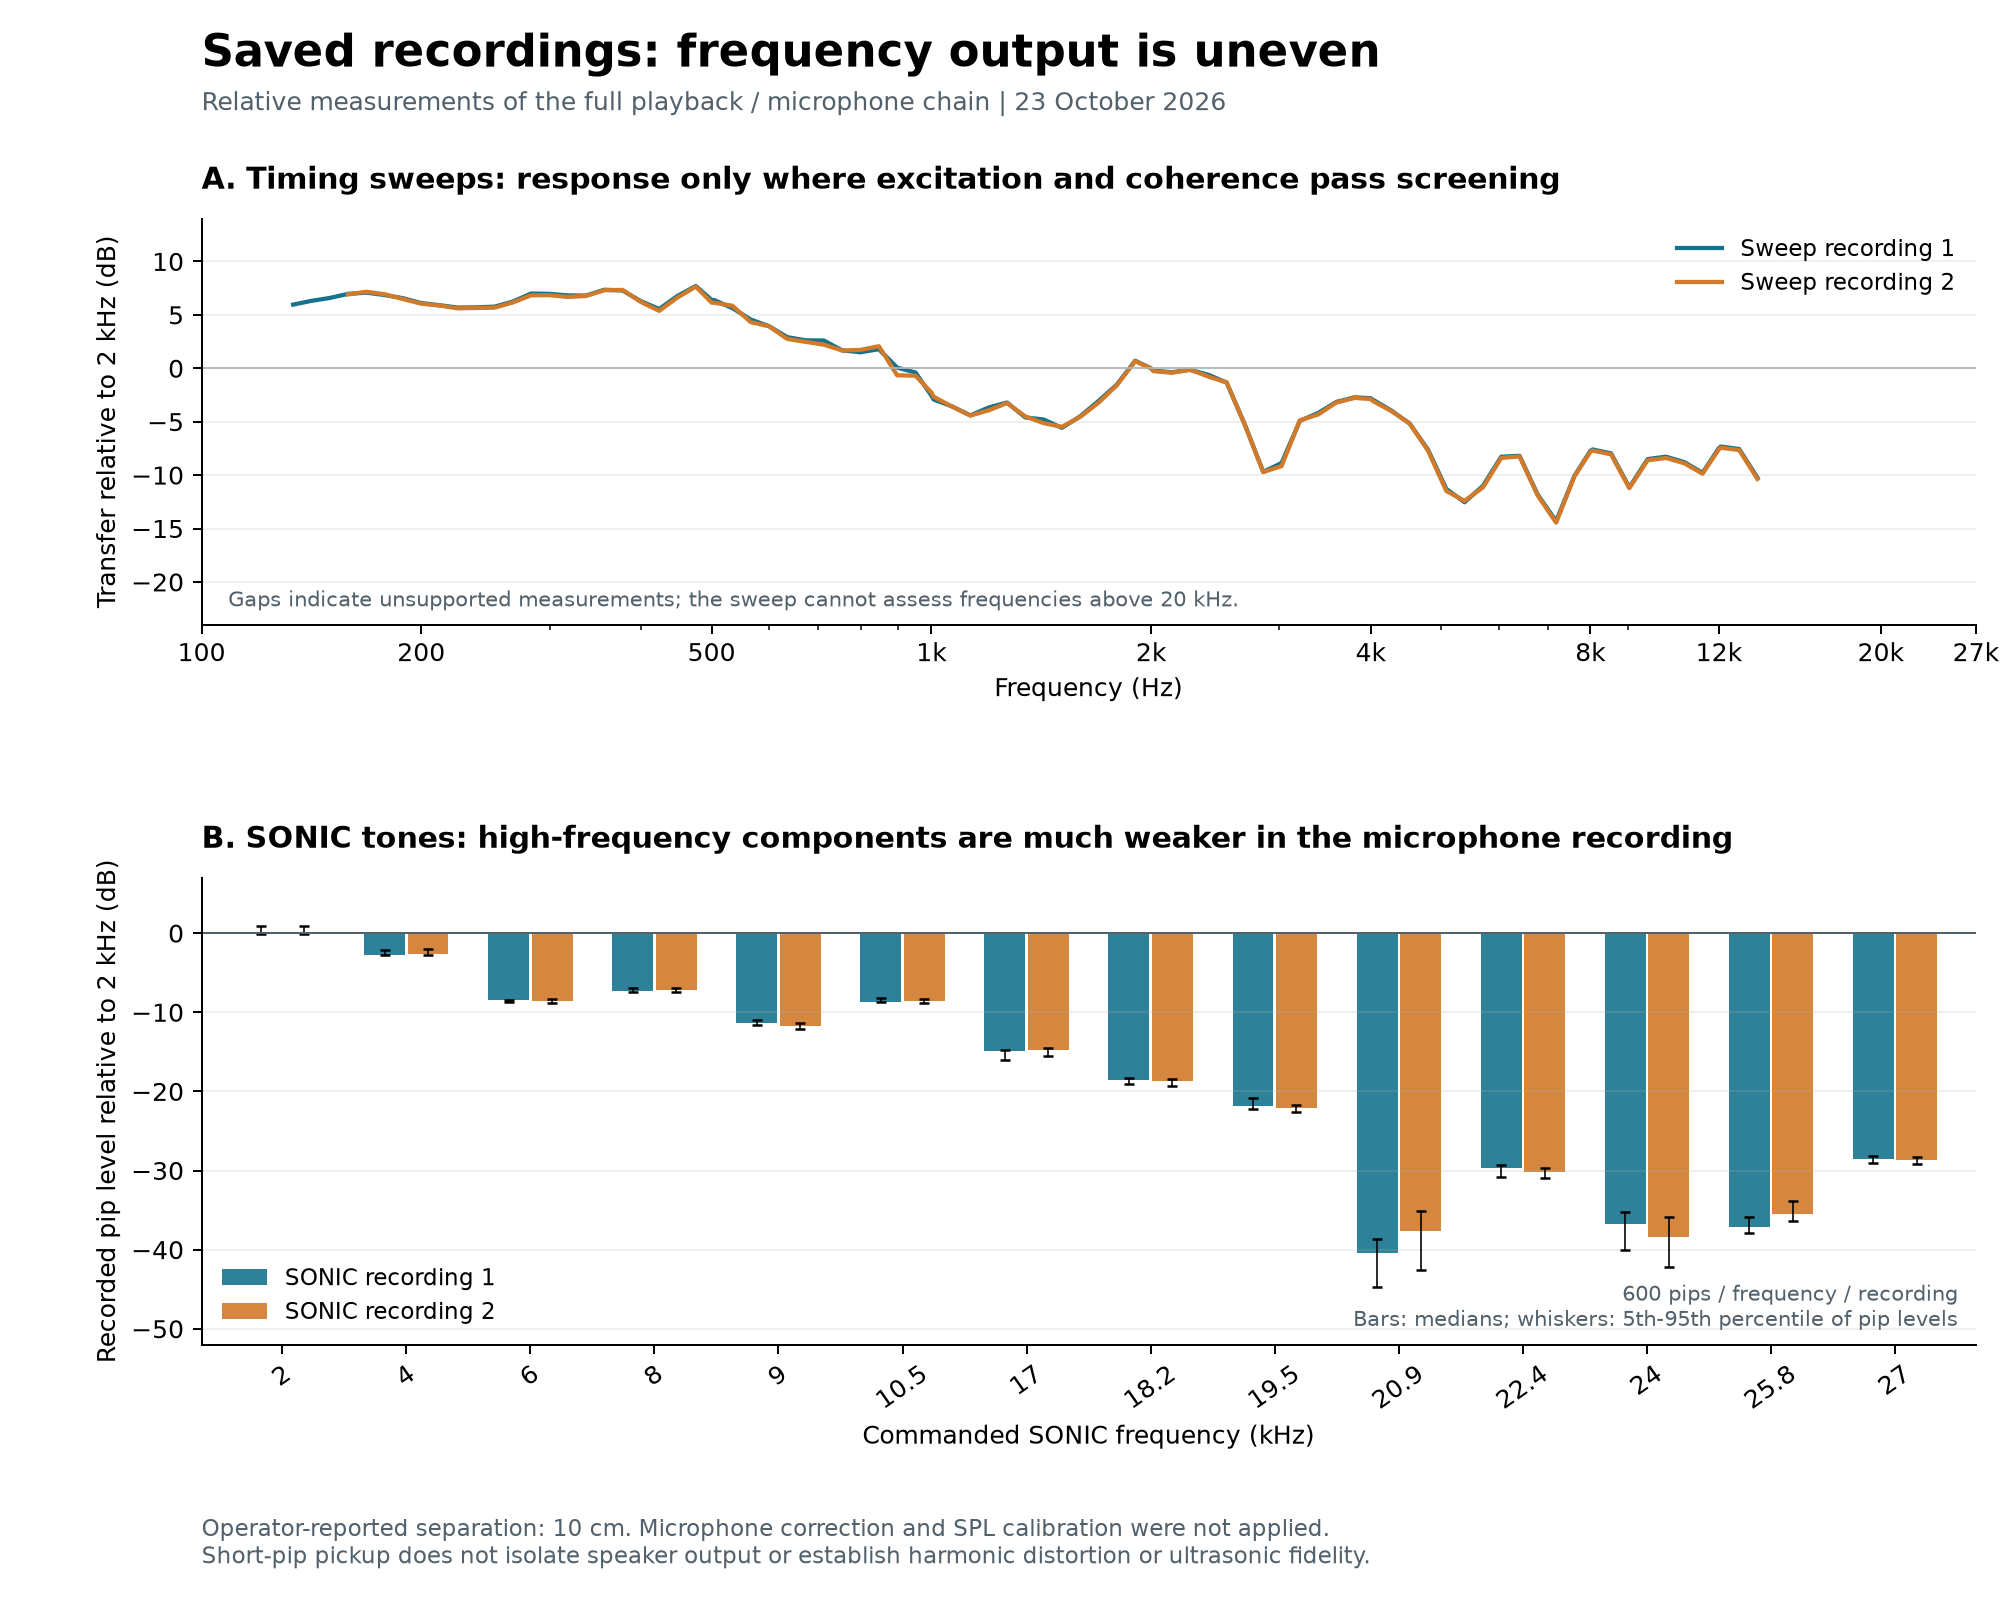
\includegraphics[width=\linewidth,height=.65\textheight,keepaspectratio]{FrequencyResponse.png}
\caption{Two independent analyses of existing recordings. Top: qualified sweep H1 magnitude bands, calculated separately for D1 and D2. Gaps are unsupported measurements. Bottom: SONIC pip component medians relative to 2\,kHz; whiskers show the within-group 5th--95th percentile spread. These are full-chain, uncorrected measurements at the saved position.}
\end{figure}

The main reproducible finding is \textbf{uneven recorded level}. Relative to
2\,kHz, the 2--10.5\,kHz groups span about 0--12\,dB attenuation; 17--19.5\,kHz
are about 15--22\,dB lower; 20.9--25.8\,kHz about 30--40\,dB lower; and 27\,kHz
about 29\,dB lower. The weak groups show more run/alignment sensitivity. Equal
digital peaks therefore cannot be treated as equal acoustic presentation levels.

At matching frequencies and times, input-1 component medians exceeded input-2
values by approximately 57--97\,dB, and input 2 showed no corresponding
event-specific rise over its pre-block floor. This is supporting comparator
evidence, not proof of acoustic origin: input gains/wiring differ, and no
speaker-disconnected isolation capture was made. The results do not isolate
speaker response from room reflections, microphone response, routing or geometry.

\newpage
\section{Relative response from the timing sweeps}
For each run independently, 0.5-second rectangular windows from $-0.1$ to
$+0.4$\,s relative to each probe onset include the source sweep and delayed
microphone response in the same flat window. A full Hann window was avoided
because delay would move the source and response onto different amplitude weights.
With averages over the 20 repeated probes,
\[
H_1(f)=\frac{\langle Y(f)X^*(f)\rangle}{\langle|X(f)|^2\rangle},\qquad
\gamma^2(f)=\frac{|\langle Y(f)X^*(f)\rangle|^2}
{\langle|X(f)|^2\rangle\langle|Y(f)|^2\rangle}.
\]
Source-power-weighted RMS magnitudes and magnitude-squared coherence were
summarized in 1/12-octave bands; levels were normalized to the qualified 2\,kHz
band. Coherent response was compared with a source-silent 0.1--0.6\,s baseline.
The local masks require coherence $\geq0.90$, source mean-bin power within
30\,dB of the strongest comparable band, response at least 10\,dB above baseline,
and valid unclipped transport. Pip phase-concentration diagnostics are different
from this cross-spectral coherence and should not be interpreted interchangeably.

\begin{table}[H]
\centering\small
\begin{tabular}{@{}rrrrrl@{}}
\toprule
kHz & D1 (dB) & D2 (dB) & $\gamma^2_1$ & $\gamma^2_2$ & Screen \\
\midrule
0.1 & -- & -- & 0.425 & 0.321 & Masked \\
0.2 & 6.10 & 6.05 & 0.998 & 0.998 & Pass \\
0.5 & 6.40 & 6.15 & 0.991 & 0.992 & Pass \\
1 & -2.53 & -2.26 & 0.975 & 0.968 & Pass \\
2 & 0.00 & 0.00 & 0.996 & 0.997 & Pass \\
4 & -2.81 & -2.87 & 0.993 & 0.994 & Pass \\
8 & -7.75 & -7.85 & 0.980 & 0.977 & Pass \\
12 & -7.50 & -7.62 & 0.950 & 0.949 & Pass \\
16 & -- & -- & 0.671 & 0.621 & Masked \\
18 & -- & -- & 0.115 & 0.114 & Masked \\
20 & -- & -- & 0.046 & 0.052 & Masked \\
\bottomrule
\end{tabular}

\caption{Representative 1/12-octave H1 band summaries relative to 2\,kHz. A dash means masked, not zero gain. Coherence alone is insufficient; excitation and baseline conditions must pass as well.}
\end{table}

\AcceptedSweepBands\ of \TotalSweepBands\ tested centers passed in both runs,
from \SupportedLowHz\,Hz through \SupportedHighHz\,Hz. The qualified combined
magnitudes span approximately 22.05\,dB. No physical bandwidth cutoff is inferred
from those endpoints. The sweep's final 20\,ms fade covers roughly 6.93--20\,kHz;
near 20\,kHz source power is extremely weak. Naive division there would create
misleading high-frequency gain. The 100\,Hz and 16/18/20\,kHz anchors are masked.

Complex spectra were not averaged across the two stream starts: their 0.125\,ms
offset would itself create phase cancellation. Each run has its own $H_1$; only
qualified magnitude summaries are compared or pooled. Finite window length,
synchronous background noise, time-varying conditions and response outside the
window remain possible biases. This is a linear relative-response screen at one
digital peak, not a THD, compression or speaker-only calibration \cite{sweep}.

\newpage
\section{SONIC sequence example and experimental meaning}
\begin{figure}[H]
\centering
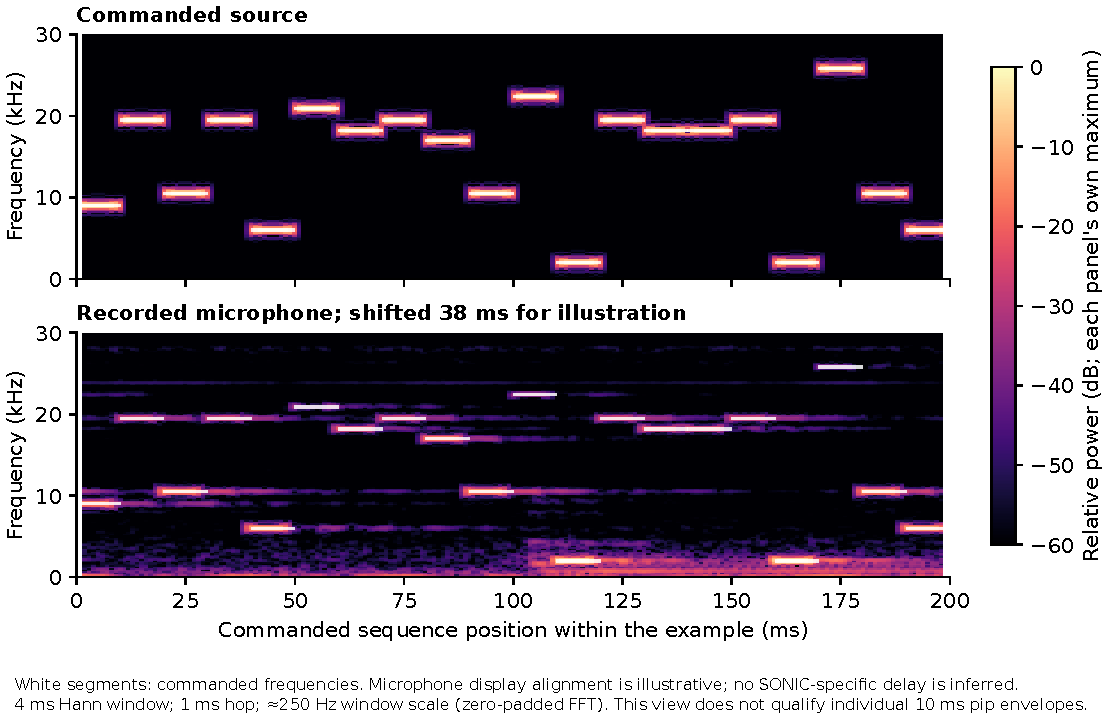
\includegraphics[width=.94\linewidth,height=.45\textheight,keepaspectratio]{SONICExample.pdf}
\caption{Actual 200-ms excerpt from S1. Commanded frequencies are shown with a microphone time--frequency display. The microphone display is shifted by approximately 38\,ms to locate content, not to establish SONIC latency. The 4-ms Hann window has a 250-Hz inverse-window scale and a broader mainlobe; the hop is 1\,ms. The view does not resolve exact acoustic onset or certify every high-frequency pip.}
\end{figure}

\subsection{What carries over from the paper}
The local reconstruction reproduces Sheep E's listed frequency alphabet, 10\,ms
pip duration, zero starting phase, 2\,ms end-ramp duration and consecutive
presentation. The paper used precomputed waveforms at 192\,kHz through an NI
USB-6361, TDT SA1 and MF1, reporting approximately 80\,dB at sheep-ear distance.
It describes 8,000--15,000 tones per block and at least 12 blocks per session.
Our two captures replay one locally seeded 8,400-pip block at 96\,kHz on different
hardware; original order, ramp shape and digital level were not available. The
paper's ear-position level is not an established or approved local output level
\cite{sonic}.

The paper's 56/11\,ms intrinsic neural-interface delays have a different
definition: they exclude auditory physiology and computation, and the 11\,ms
result is a narrower session/window sweep. Comparing them directly with this
38.3\,ms audio application roundtrip would be invalid. No neural decoding,
physiological latency or ITR can be inferred from these bench recordings.
Published SONIC animals were awake and alert; planned Rice work in sedated sheep
is a separate adaptation whose responses remain unmeasured \cite{sonic,project}.

\newpage
\section{Limits and prioritized next bench tests}
The evidence establishes operation, short-run roundtrip repeatability and
frequency-dependent recorded pickup. It leaves \textbf{absolute SPL, isolated
speaker fidelity, distortion, physical onset and neural-clock alignment open}.
The M50 has a serial-specific calibration file; none was applied here. Nominal
manufacturer bandwidth or sensitivity cannot replace calibration of the delivered
microphone, preamp gain and complete acoustic geometry \cite{m50}.

The 96\,kHz stream has a 48\,kHz Nyquist frequency, so a 27\,kHz fundamental is
representable in principle. Its 54\,kHz second harmonic is not. At 24\,kHz the
second harmonic lies at Nyquist; higher tones have second harmonics above it.
Faster conversion alone would still require calibrated microphone and analog
front-end coverage. Short continuous pips also mix source-window leakage,
neighboring tones and ringing, so these recordings do not provide full THD or
THD+N. No numeric flatness, level, distortion or onset tolerance has been approved.

\begin{table}[H]
\small
\begin{tabularx}{\linewidth}{@{}P{.06\linewidth}P{.25\linewidth}Y@{}}
\toprule
Order & Proposed next test & Evidence required before closing the question\\
\midrule
1 & Fix the physical configuration & Record the active cabinet/channel, reference plane, tip position and angle, room/background, gains, EQ, routing, sample rate and firmware version. Use the intended measurement position.\\
2 & Calibrate the measurement chain & Load the serial-matched M50 correction and establish level conversion with a suitable acoustic reference at the recorded gain. Target SPL and convention: TBD with Dr. Luan.\\
3 & Isolate acoustic pickup & Compare playback with the speaker path active and silent/disconnected while retaining interface/microphone connections. Quantify residual electrical feedthrough.\\
4 & Measure each frequency separately & Use settled, separated tones across all 14 frequencies, repeated orders and documented digital levels. Assess response, noise, ringing and measurable harmonic orders. Level/flatness/distortion tolerances: TBD.\\
5 & Validate independent timing & Establish a known electrical return alongside the microphone, verify channel skew, and repeat stream starts, buffer settings and longer captures. Timing accuracy/jitter requirement: TBD.\\
6 & Integrate the neural timebase & Validate the eventual trigger/clock mapping to the neural recorder. Confirm the animal-position acoustic stimulus before interpreting neural response windows. No animal work is established by this report.\\
\bottomrule
\end{tabularx}
\caption{Proposed validation sequence, not tests already performed. Suggested bench owner: Howard; experimental targets and acceptance criteria: TBD with Dr. Luan. No purchase, exposure level, procedure or animal protocol is approved here.}
\end{table}

The immediate decision is to retain the working setup for controlled bench
characterization, while treating full-band level uniformity and calibrated timing
as open measurements. The present high-frequency attenuation does not identify
a defective component: speaker directivity, two-cabinet interference, position,
room response, hardware settings and microphone correction remain hypotheses to test.

\newpage
\section{Reproducibility and evidence ledger}
The numeric tables are generated from the saved verification records, rather
than manually entered. A fresh offline audit reproduced both timing/H1 analyses
and both pip analyses and matched all 34 checked SHA-256 references. Figures use
actual saved samples or measured aggregate values; synthetic signals are used
only in software tests. Original raw arrays, timestamps and manifests remain
local under ignored \path{.work/latency/runs/}.

\textbf{Provenance files.} \path{data-manifest.json} records the verification-file,
code and pinned-paper hashes. \path{images/figures-manifest.json} records exact
source windows, normalization, STFT settings and raw/figure hashes. These accompany
the editable LaTeX project. The pinned paper stays unchanged with its version,
checksum and CC BY-NC-ND 4.0 notice; all plotted experimental figures are local data.

\textbf{Historical records retain their original scope.} Earlier silent/weak
microphone checks and missing electrical-return analyses did not establish a delay.
The later source-array roundtrip does not retroactively validate input 2. D2's
initial manifest omitted a native-acquisition flag; the original was retained as
\path{manifest.as-acquired.json}, and the documented metadata amendment added that
flag without changing audio or timestamps \cite{delay}.

\textbf{Offline reproduction} (requires the private saved captures):
\begin{quote}\small\ttfamily
python -m latency.roundtrip --analyze-run RUN\_FOLDER\\
python -m latency.pip\_response\\
python -m latency.sweep\_response\\
python scripts/create\_frequency\_response\_figure.py\\
python scripts/create\_full\_bench\_report\_data.py\\
python scripts/create\_full\_bench\_report\_figures.py
\end{quote}
These analysis/figure commands do not play sound. Compile this project's
\path{main.tex} to regenerate the report. The dataset is small, covers two
stream starts per stimulus family and repeats the same source sequences; no
long-term or independent-session confidence interval is claimed.

\begingroup\footnotesize
\begin{thebibliography}{99}
\bibitem{sonic} \emph{SONIC: A Benchmarking Paradigm for Brain-Computer Interfaces}.
bioRxiv v1, posted 2 October 2025. Methods 6.1--6.2 (p.\ 11), animal state 6.6
(p.\ 13), intrinsic-delay results (pp.\ 5, 7--8).
\url{https://doi.org/10.1101/2025.09.30.679683}.
\bibitem{delay} Project measured timing record, 23 October 2026.
\url{https://github.com/HowardWHSrun/audiotory_benchmark/blob/main/docs/verification/2026-10-23_Audient_Playback_Microphone_Delay.json}.
\bibitem{pip} Project two-capture E14 pip-frequency review, 23 October 2026.
\url{https://github.com/HowardWHSrun/audiotory_benchmark/blob/main/docs/verification/2026-10-23_SONIC_E14_Pip_Frequency_Pickup.json}.
\bibitem{sweep} Project screened sweep H1 response, 23 October 2026.
\url{https://github.com/HowardWHSrun/audiotory_benchmark/blob/main/docs/verification/2026-10-23_Sweep_Relative_Response.json}.
\bibitem{basic} Project basic playback/recording verification.
\url{https://github.com/HowardWHSrun/audiotory_benchmark/blob/main/docs/verification/2026-10-23_Audient_Basic_Playback_Recording.json}.
\bibitem{playback} Project E14 playback and unqualified direct-tone timing review.
\url{https://github.com/HowardWHSrun/audiotory_benchmark/blob/main/docs/verification/2026-10-23_SONIC_E14_Playback.json}.
\bibitem{portaudio} PortAudio, \emph{Buffering, Latency and Timing Implementation Guidelines}
(draft guidance), accessed 23 October 2026.
\url{https://github.com/PortAudio/portaudio/wiki/BufferingLatencyAndTimingImplementationGuidelines}.
\bibitem{ni} NI, \emph{Understanding FFTs and Windowing}, accessed 23 October 2026.
\url{https://www.ni.com/en/shop/data-acquisition/measurement-fundamentals/analog-fundamentals/understanding-ffts-and-windowing.html}.
\bibitem{m50} Earthworks Audio, M50 specifications and individual electronic calibration file,
accessed 23 October 2026. \url{https://earthworksaudio.com/measurement-microphones/m50/}.
\bibitem{project} Project working directions: planned Rice sedated-sheep adaptation.
\url{https://github.com/HowardWHSrun/audiotory_benchmark/blob/main/AGENTS.md}.
\end{thebibliography}
\endgroup
\end{document}
